\chapter{Resultados Práticos}

Este capítulo abordará os resultados práticos obtidos durante o desenvolvimento deste trabalho.

\section{Montagem da Planta}

Como relatado na Seção \ref{sec:EstruturaCAD}, ao se desenhar as placas da estrutura em \textit{software} CAD levou-se em consideração os furos para os componentes e passagem das cablagens. Em relação ao material, as mesmas são de ACM preto e foram cortadas por uma fresadora para um melhor acabamento e precisão. A Figura (\ref{fig:vistasMontagemPlanta}) mostra duas vistas da montagem, frontal e lateral. Além da estrutura mecânica, é visto também o conjunto de motores e rodas e os componentes eletrônicos.

\begin{figure}[H]
\centering
\includegraphics[width=8cm]{Resultados/MontagemFrontal.png}
\includegraphics[width=8cm]{Resultados/MontagemLateral.png}
\caption{Vistas frontal e lateral da montagem da planta física.}
\label{fig:vistasMontagemPlanta} 
\end{figure}

\section{Validação do Sensor e Motores}

Com a finalização da construção da planta física, projeto do controlador e realização da simulação conforme mostrado no Capítulo \ref{cap:ModelagemProjetoControlador}, foram realizados testes práticos para verificação do funcionamento do sistema montado. Foi desenvolvido um código utilizando a linguagem C, uma vez que a placa controladora será o microcontrolador Arduino. Essa placa tem como principal responsabilidade o processamento do sinal do sensor de posição angular para obtenção do sinal de controle utilizando dos ganhos do controlador LQG e consequentemente, gerando um sinal PWM para a placa L298N acionar os motores de corrente contínua. O código desenvolvido está em meu \href{https://github.com/mferreiracosta/tcc_cefet.git}{github}, mas a ideia de funcionamento é, basicamente:

\begin{itemize}
    \item se a estrutura tender a ir para frente, os motores receberão um valor de PWM e um comando para ir para frente. O valor do PWM é dependente de uma multiplicação matricial do valor do sinal do sensor filtrado e do ganho do regulador linear quadrático.
    \item caso a estrutura for para trás, o comando que a placa L298N receberá será contrário aquele recebido quando a estrutura for para frente. A lógica cálculo do valor do PWM se mantém a mesma.
\end{itemize}

Após desenvolvimento do código, esse foi carregado para o Arduino para obtenção dos sinais do sensor e acionamento dos motores para testes de movimentação. O circuito eletrônico montado tanto para testes quanto para controle da posição do pêndulo está esquematizado na Figura (\ref{fig:circuitoEletronicoPlanta}). Os resultados são visto abaixo.

\subsection{Validação do Sensor}

Após a montagem do circuito eletrônico, como mostrado acima na Figura (\ref{fig:circuitoEletronicoPlanta}), desenvolvimento do código Arduino e carregamento do mesmo na placa, foi possível realizar as validações. Primeiramente, focou-se em validar os sinais do sensor. A ideia é ver a diferença entre o sinal real do sensor e o filtrado por Kalman, afim de corroborar com o que a literatura afirma a respeito deste filtro, de que o mesmo traz uma maior robustez e é menos sensível a ruídos e distúrbios.

Entretanto, para obter os dados do sensor só foi possível através da serial da porta do computador, uma vez que neste trabalho não se utiliza de nenhum componente eletrônico de transmissão. Sendo assim, desenvolveu-se um código no Processing, o qual fez a leitura dos dados em forma de \textit{string} da serial e os salvaram em um arquivo ``.txt". Com esse arquivo, desenvolveu novamente um novo código, só que dessa vez foi utilizando a linguagem Python. Dessa maneira, realizou-se os tratamentos necessários e gerou-se as figuras com os resultados obtidos.

Com intuito de validar bem os sinais e o filtro desenvolvido, gerou-se mais de um arquivo com dados. De forma macro, a Figura (\ref{fig:sinaisMacroSensor}), mostra o resultado guardado de dois arquivos. O interessante desse resultado visto, é observar que o sinal real (\textit{pitch}) é bastante sensível a ruído e o sinal filtrado, por sua vez, é bem suave mas sempre segue o sinal real.

\begin{figure}[H]
\centering
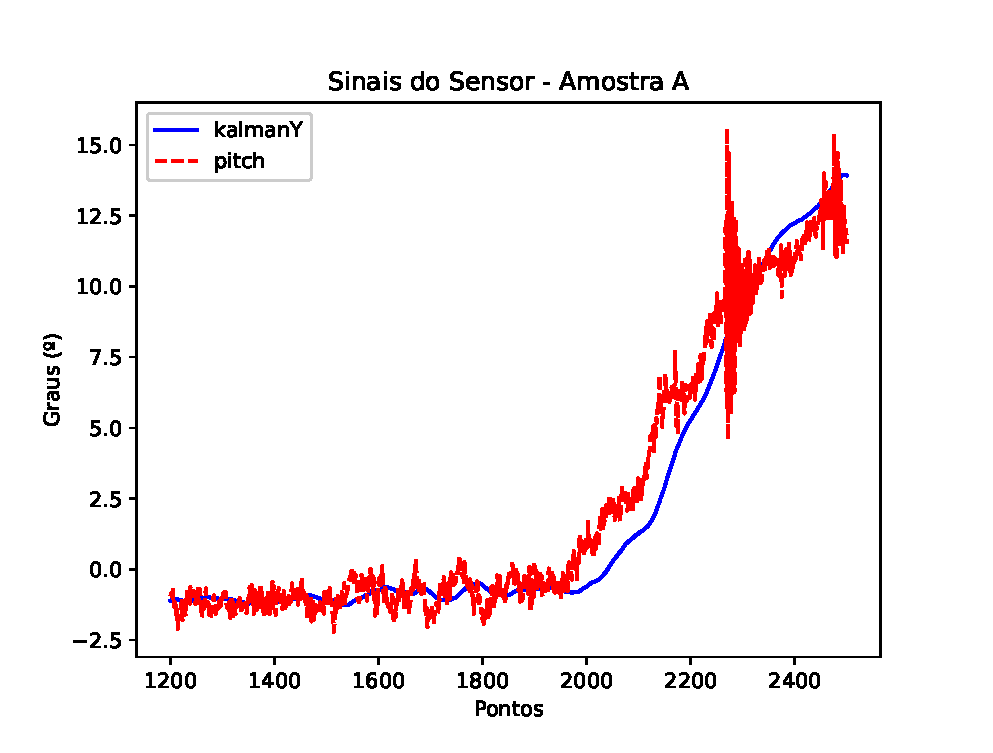
\includegraphics[width=8cm]{Resultados/sinaisAmostraA.eps}
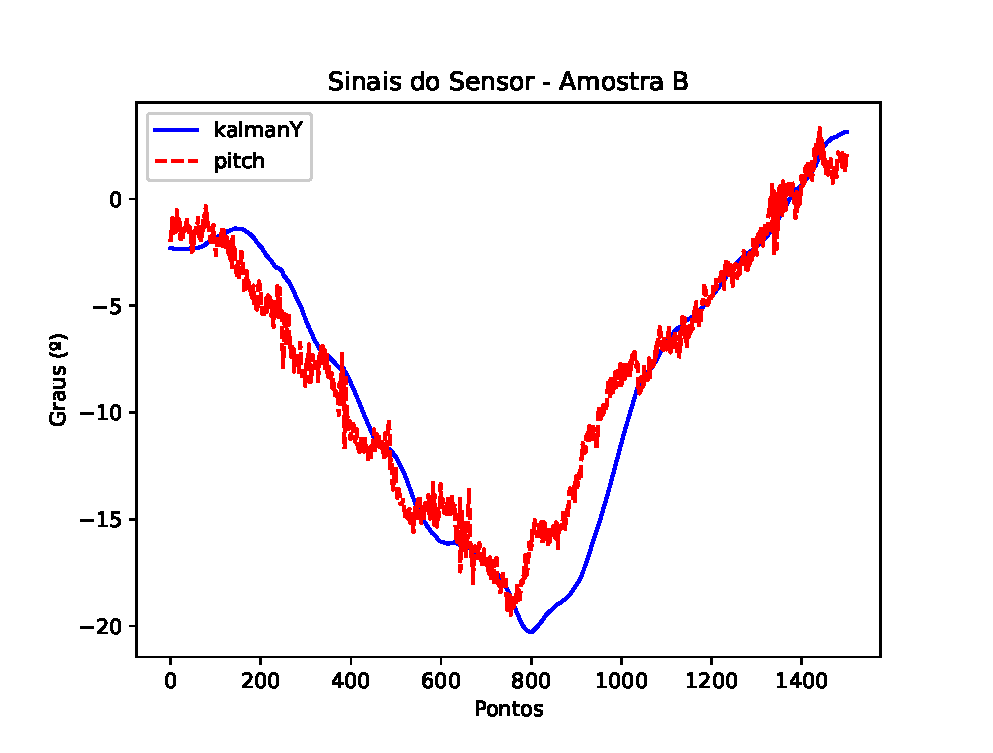
\includegraphics[width=8cm]{Resultados/sinaisAmostraB.eps}
\caption{Comportamento de forma macro do sinal do sensor filtrado, curva azul e do sinal real, curva vermelha.}
\label{fig:sinaisMacroSensor} 
\end{figure}

Para uma melhor visualização da curva, plotou-se apenas uma pequena fatia dos dados da amostra B, como mostra a Figura (\ref{fig:sinaisFatiadoSensor}). Aqui, verifica-se e comprova o que foi dito, que a sensibilidade a ruído do sinal real é bem alta e que o sinal filtrado segue a curva real de forma bem suave.

\begin{figure}[H]
\centering
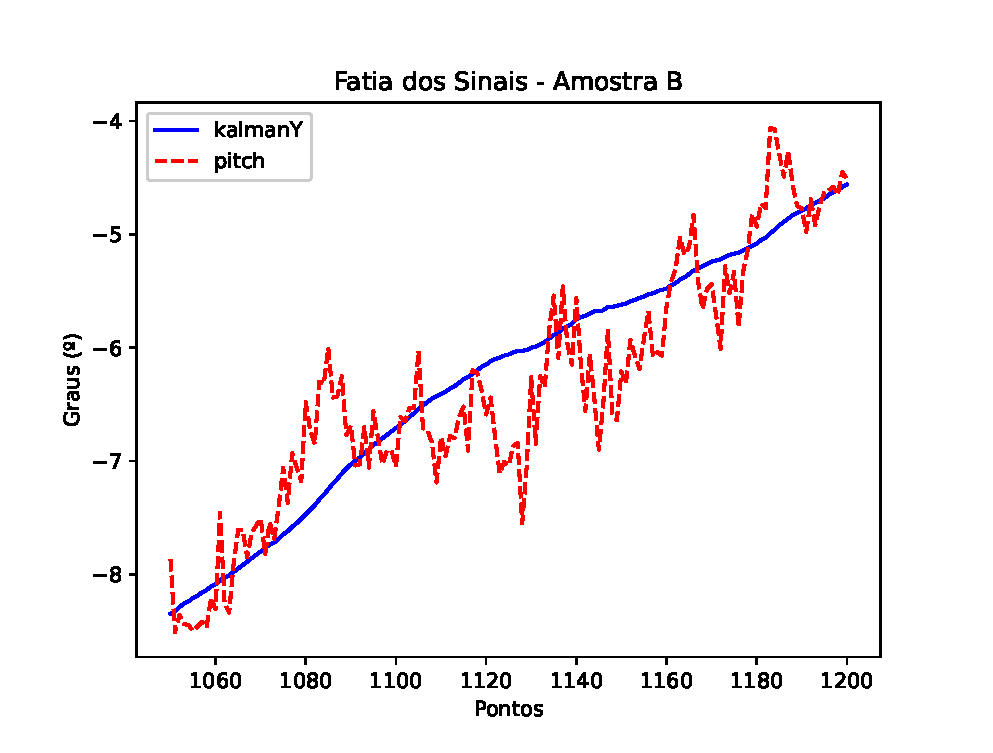
\includegraphics[scale=0.75]{Resultados/fatiaSinalSensor.eps}
\caption{Comportamento de forma micro dos dois sinais do sensor.}
\label{fig:sinaisFatiadoSensor} 
\end{figure}

\subsection{Validação dos Motores}

\section{Aplicação do Controlador}

